\documentclass{article}

\usepackage{graphicx}
\usepackage{tikz}
\usepackage{tikzsymbols}
\usetikzlibrary{calc,patterns,shapes.geometric}
\pagestyle{empty}
\usepackage[margin=0pt]{geometry}
\geometry{papersize={14in,12in}}

\def\centerarc[#1](#2)(#3:#4:#5){\draw[#1] ($(#2)+({#5*cos(#3)},{#5*sin(#3)})$) arc (#3:#4:#5);}

\begin{document}
	\begin{figure}
		\centering
		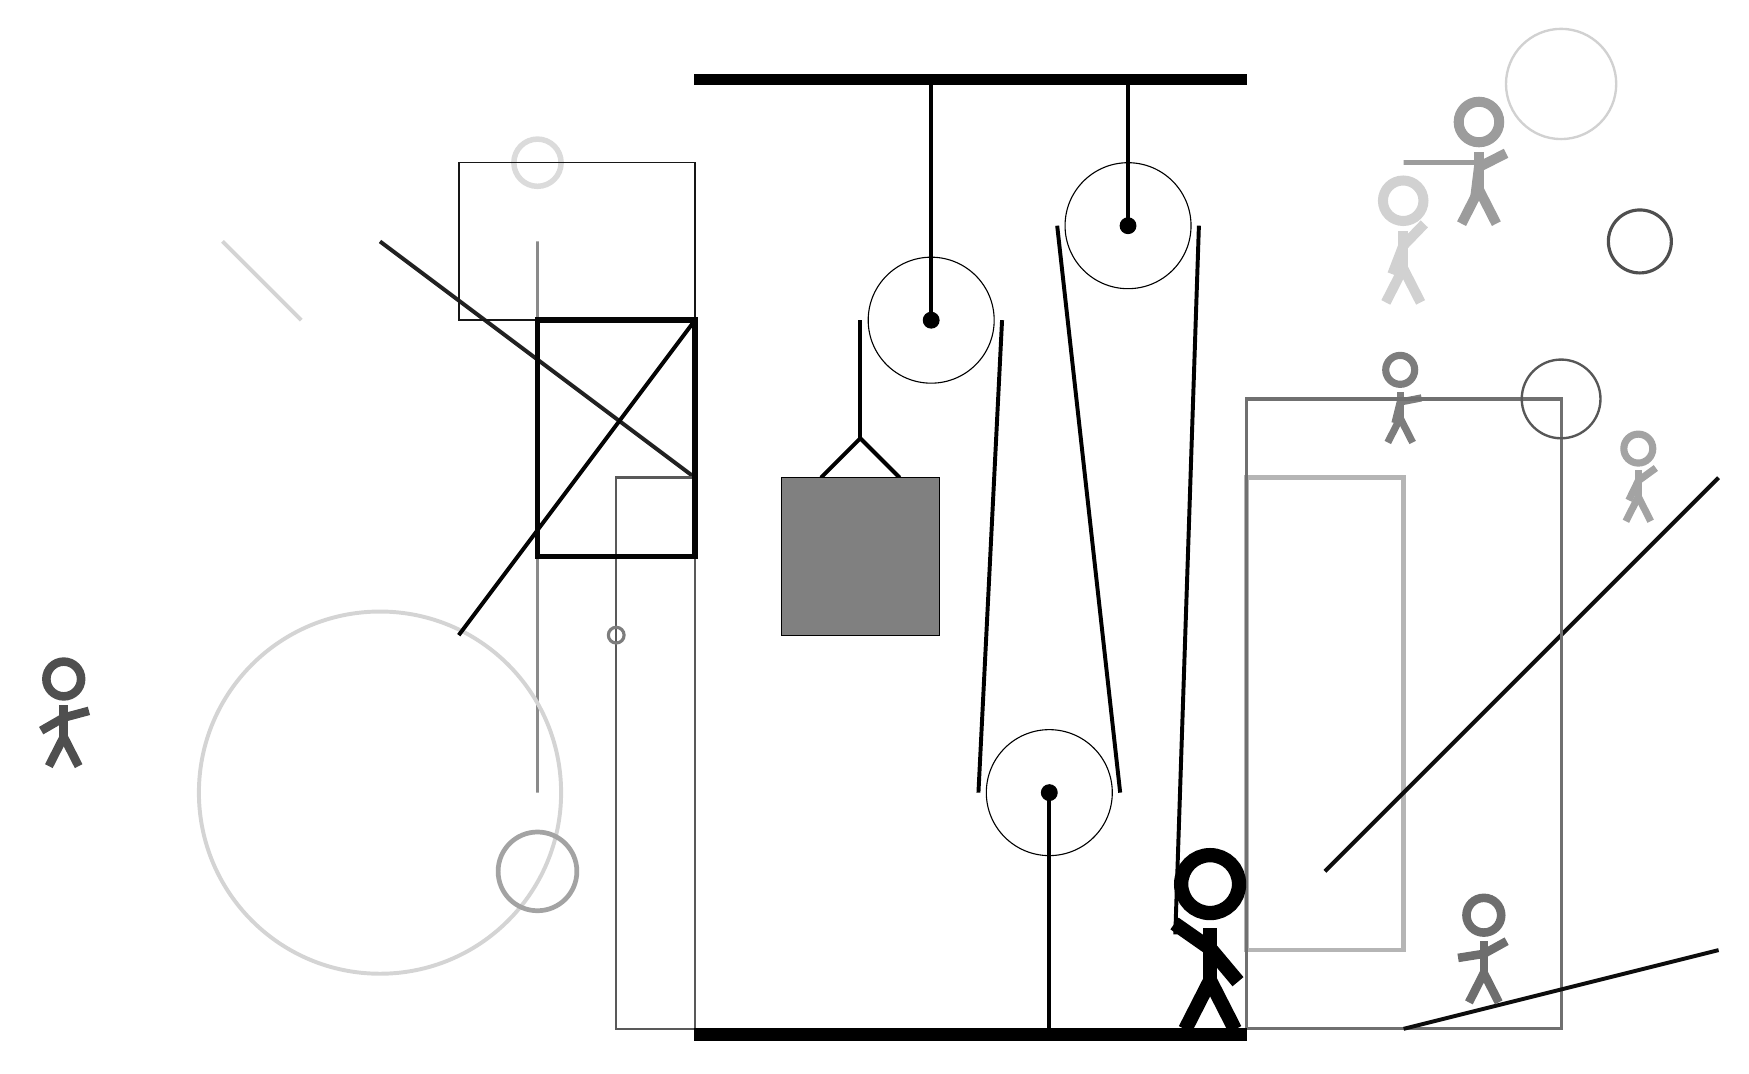
\begin{tikzpicture}
			%%%%% START %%%%%
			
			\draw[fill=black] (-2, 9) rectangle (5, 9.125);
			
			\draw (1, 6) circle (0.8);
			\draw[fill=black] (1, 6) circle (0.1);
			\draw[line width=0.5mm]  (1, 9) -- (1, 6);
			
			\node[line width=0.3mm, color=black!39] at (8, 8) {\Strichmaxerl[7][83][27]};
			
			\draw[line width=0.6mm, color=black!29] (7, -2) rectangle (5, 4);
			\draw [line width=0.7mm, color=black!90](-3, 4) circle (0.0);
			\draw[line width=0.4mm, color=black!46] (-4, 0) rectangle (-4, 7);
			
			\draw [line width=0.4mm, color=black!69](10, 7) circle (0.4);
			
			\node[line width=0.3mm, color=black!69] at (-10, 1) {\Strichmaxerl[6][30][15]};
			\node[line width=0.2mm, color=black!51] at (7, 5) {\Strichmaxerl[5][76][11]};
			\draw[line width=0.5mm, color=black!87](-6, 7) -- (-2, 4);
			\draw [line width=0.5mm, color=black!17](-6, 0) circle (2.3);
			\draw [line width=0.3mm, color=black!18](9, 9) circle (0.7);
			
			\draw [line width=0.7mm, color=black!14](-4, 8) circle (0.3);
			\node[line width=0.6mm, color=black!18] at (7, 7) {\Strichmaxerl[7][69][46]};
			\draw[line width=0.5mm, color=black!95](6, -1) -- (11, 4);
			\draw[line width=0.5mm, color=black!17](-7, 6) -- (-8, 7);
			\draw[line width=0.4mm, color=black!56] (5, -3) rectangle (9, 5);
			\draw[line width=0.2mm, color=black!91] (-2, 6) rectangle (-5, 8);
			
			\draw [line width=0.3mm, color=black!66](9, 5) circle (0.5);
			\draw[line width=0.5mm, color=black!99](-2, 6) -- (-5, 2);
			\draw[line width=0.5mm, color=black!95](7, -3) -- (11, -2);
			\draw [line width=0.6mm, color=black!36](-4, -1) circle (0.5);
			\node[line width=0.5mm, color=black!57] at (8, -2) {\Strichmaxerl[6][9][29]};
			
			\draw[line width=0.3mm, color=black!65] (-2, -3) rectangle (-3, 4);
			
			\node[line width=0.4mm, color=black!36] at (10, 4) {\Strichmaxerl[5][64][36]};
			\draw [line width=0.4mm, color=black!51](-3, 2) circle (0.1);
			\draw[line width=0.7mm, color=black!98] (-2, 6) rectangle (-4, 3);
			\draw[line width=0.6mm, color=black!39] (7, 8) rectangle (8, 8);
			
			\draw[fill=white](2.5, 0) circle (0.8);
			\draw[fill=black] (2.5, 0) circle (0.1);
			\draw[line width=0.5mm]  (2.5, -3) -- (2.5, 0);
			
			\draw[fill=white](3.5, 7.2) circle (0.8);
			\draw[fill=black] (3.5, 7.2) circle (0.1);
			\draw[line width=0.5mm] (3.5, 9) -- (3.5, 7.2);
			
			\draw[line width=0.5mm] (-0.4, 4.0) -- (0.1, 4.5) -- (0.6, 4.0);
			\draw[fill=black!50] (-0.9, 4.0) rectangle (1.1, 2.0);
			
			\draw[line width=0.5mm] (0.1, 6) -- (0.1, 4.5);
			\centerarc[line width=0.5mm](1, 6)(0:180:0.9);
			\draw[line width=0.5mm](1.9, 6) -- (1.6, 0);
			\centerarc[line width=0.5mm](2.5, 0)(180:360:0.9);
			\draw[line width=0.5mm](3.4, 0) -- (2.6, 7.2);
			\centerarc[line width=0.5mm](3.5, 7.2)(0:180:0.9);
			\draw[line width=0.5mm](4.4, 7.2) -- (4.1, -1.8);
			
			\node at (4.5, -1.9) {\Strichmaxerl[10][-35][-50]};
			
			\draw[fill=black] (-2, -3) rectangle (5, -3.15);
			
			%%%%% END %%%%%
		\end{tikzpicture}
	\end{figure}	
\end{document}